\documentclass{beamer}
%===============
%PACKAGE UTILISE
%===============
\usepackage[size=a0, orientation=landscape, scale=1.4]{beamerposter}
\usepackage[utf8]{inputenc}
\usepackage[T1]{fontenc}
\usepackage[french]{babel}

\usepackage{graphicx}
\usepackage{wrapfig}
\usepackage{listings, xcolor, soul}

%=====definition des couleurs utilisées===
\definecolor{blancCreme}{RGB}{247,255,255}
%\usepackage{xcolor, soul}
\sethlcolor{orange}

%===========
%BAS DE PAGE
%===========
\title[Rapport]{La reconnaissance facial}
\subtitle[\ldots]{Rapport}
\author{Julie PRIGENT n° et Dorine HENRY n° etudiant: 20192366}
\institute[Evry]{Evry Val d'Essonne}

%====
%BODY
%====
\begin{document}

%\logoright{
\includegraphics[height=7cm]{logoEvry.jpg}}
%---------------------------------BACKGROUND-------------------------------------------------
\setbeamertemplate{background}{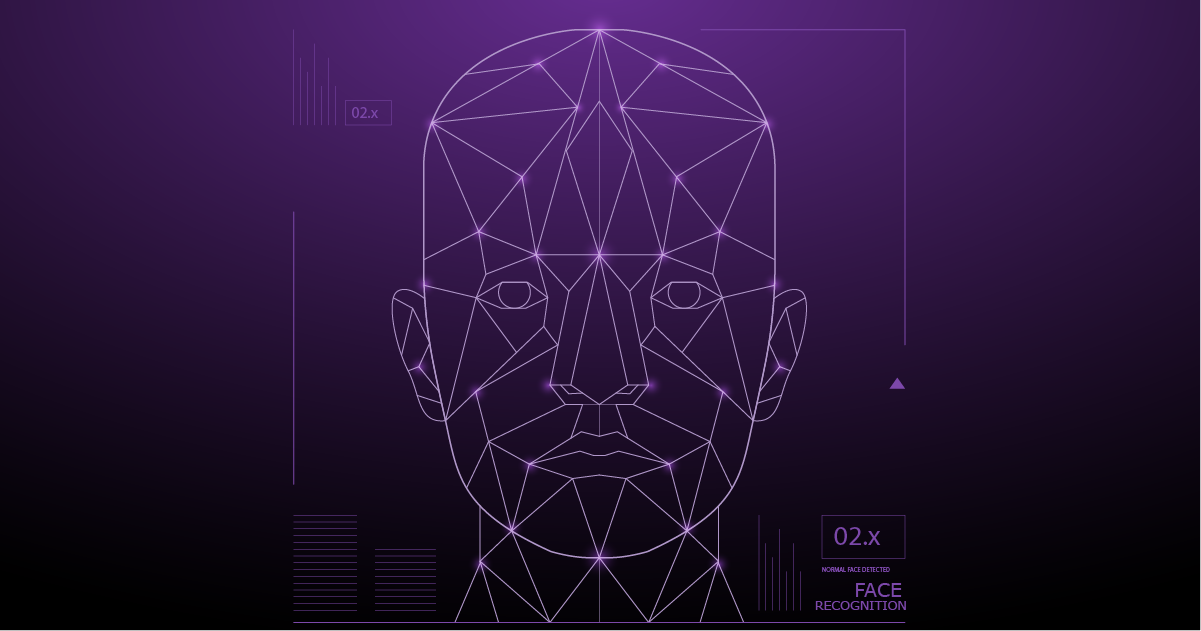
\includegraphics[height=\paperheight]{background.png}}
 
\begin{columns}[c]
    \begin{column}{0.5\textwidth}
    \color{blancCreme}
%------------------------------------TITRE---------------------------------------------------
\hrulefill 
   \Huge{ LaTeX \quad \hrulefill {\bf La reconnaissance faciale} \hrulefill Rapport PPEI } \par
   	\hrulefill
    \end{column}
\end{columns}

\begin{columns}[c]	 
	\begin{column}{0.5\textwidth}
	\color{blancCreme}
%-------------------------------introduction ------------------------------------------------
  	 {\bf Introduction:} \\
Pour déverrouiller son téléphone, retrouver une personne disparue ou encore déduire l’avis d’un client à partir de ses expressions faciales, la reconnaissance faciale rythme nos vies et fait l’objet de nombreuses recherches et investissements.\\ Quelles sont les particularités des algorithmes sur lesquels cette technologie est fondée ? \par
	\hrulefill
	\end{column}
\end{columns}
	
\begin{columns}[c]
	
	\begin{column}{.46\textwidth}
	\color{blancCreme}
%----------------------------detection du visage---------------------------------------------
	{\bf Detection du visage :}\\
     Pour avoir recours à la reconnaissance faciale nous faisons appel à des algorithmes qui doivent tout d’abord déterminer la position d’un visage sur une image donnée. Lorsque l’on soumet une image à un de ces algorithmes, il la considère comme un ensemble de pixels, caractérisés par leur intensité. L’intensité d’un pixel varie selon la luminosité,  ainsi l’algorithme transforme cette donnée en “gradient”. Pour ce faire, chaque pixel est comparé par sa valeur à ses voisins, et est remplacé par une flèche qui indique la direction vers laquelle se trouvent d’autres pixels d’intensité similaire. A ce stade l’algorithme découpe l’image en zones, pour lesquelles il va calculer un “gradient fort”, qui correspond à la moyenne des gradients contenus dans la zone. On obtient alors un histogramme de gradient (HOG). \\
L’algorithme utilise ensuite un HOG générique de visage humain, obtenu  à l’aide de machine learning. L’algorithme va chercher si le HOG générique se retrouve au sein de l’image qu’il analyse, et le cas échéant, il considérera qu’un visage humain se trouve à cet endroit. 
\par

	\begin{figure}
	\color{blancCreme}
		\caption{Schéma detection du visage}
		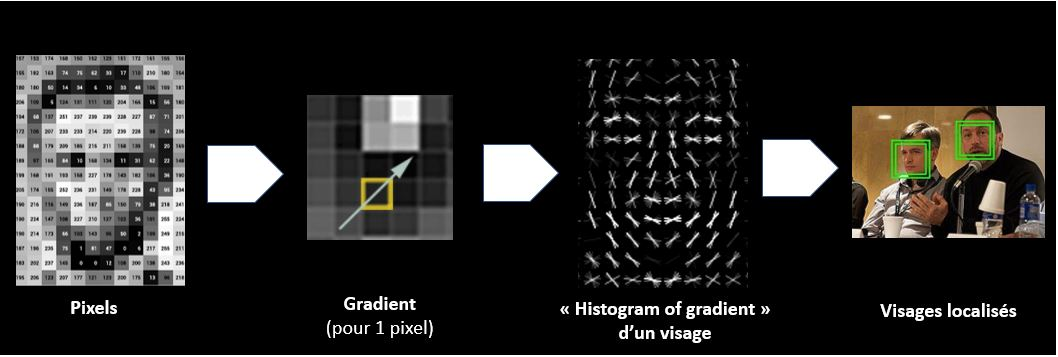
\includegraphics[width=40cm]{Localise.jpg} \par	
		\hrulefill
	\end{figure}	
	\end{column}

	\begin{column}{.4\textwidth}
	\color{blancCreme}
%---------------------------------------EXEMPLE--------------------------------------------	
	{\bf Exemple:}\\
		
	 {\bf Recherche de criminels :} Aux États-Unis les citoyens arrêtés par la police sont systématiquement pris en photos. Ces photos appelées “mug shots” sont stockées dans des bases de données sur lesquelles les agents lancent des algorithmes de reconnaissance faciale, afin de retrouver des criminels en fuite qui apparaîtraient sur des caméras de surveillance par exemple. 

	 {\bf Contrôles de papiers dans les aéroports :} De plus en plus d’aéroports proposent aux usagers de contrôler leurs papiers d’identité (dans ce cas les passeports) par un scan de leur visage. Des algorithmes de reconnaissance faciale authentifie que les documents présentés correspondent bien aux données biométriques qu’il a récolté.\par
	\hrulefill
	
	{\bf “Tromperie” sur la reconnaissance faciale:} 
Des maquillages ont été mis au point pour induire en erreur les algorithmes de reconnaissance faciale. Ceux ci créent des contrastes inhabituels pour un visage humain. Ainsi le HOG obtenu à l’emplacement du visage ne correspond plus. et l’algorithme sera incapable d’identifier qu’un visage s’y trouve.\par
	\hrulefill
	\end{column}
\end{columns}

\begin{columns}

	\begin{column}{.3\textwidth}
	\color{blancCreme}
%-----------------------------reconnaissance faciale------------------------------------ 
   {\bf Reconnaissance 2D:}\\
Une fois le visage localisé par l’algorithme, l’analyse de celui-ci débute par le positionnement sur le visage de “points spécifiques”. Ces points sont au nombre de 68 et ont été déterminés afin qu’ils se retrouvent sur tous les visages humains.  Un algorithme de machine learning se charge de les identifier sur chaque visage qui lui est soumis. A partir de ces points, l’algorithme va recadrer le visage de sorte à ce qu’il se trouve dans une position standard et puisse être comparé à tous ceux que l’algorithme à déjà traité. En comparant ce visage à ceux d’une base de donnée, l’algorithme indiquera si une correspondance a été trouvée ou non.\par
	\begin{figure}
	\color{blancCreme}
		\caption{Schéma reconnaissance 2D}
		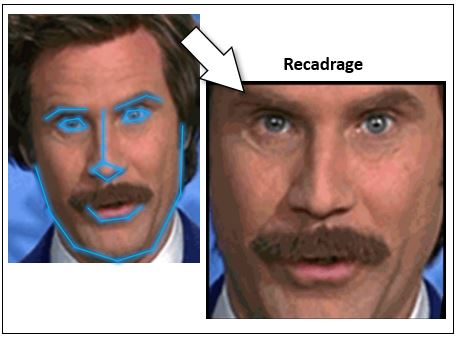
\includegraphics[width=15cm]{Reco2D.jpg}
	\end{figure}
	\end{column}
	
	\begin{column}{.3\textwidth}
	\color{blancCreme}
   {\bf Reconnaissance 3D:}\\
La reconnaissance faciale par modélisation 3D est une technologie encore peu utilisée de par les moyens matériels qu’elle demande, on la retrouve dans les Iphone avec leur système de caméra True Depth. L’appareil projette 30 000 faisceaux infrarouge sur le visage de l’utilisateur, le temps que prend l’infrarouge avant d’être reflété sur le visage permet aux algorithmes de mettre en œuvre en temps réel une modélisation 3D du visage. Celle-ci est comparée à celle établie lors de la configuration du déverrouillage par la reconnaissance faciale.\par
	\begin{figure}
	\color{blancCreme}
		\caption{Schéma reconnaissance 3D}
		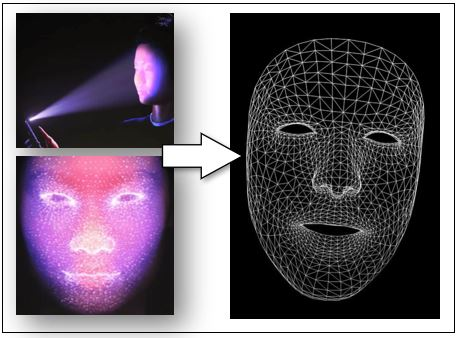
\includegraphics[width=15cm]{Reco3D.jpg}
	\end{figure}
	\end{column}
\end{columns}

\begin{columns}[t]
	\begin{column}{.9\textwidth}
	\color{blancCreme}
%-----------------------------CONCLUSION----------------------------------------------------
	{\bf Conclusion:}\\
   	La reconnaissance faciale fait appel à de l’intelligence artificielle. Pour que ces modèles soient performants, ils doivent être entraînés sur des bases de données contenant des milliers d’images de visages, parfois récupérées sur les réseaux sociaux sans que les utilisateurs en soient avertis. Ce qui pose des questions sur la sécurité des données personnelles.\par
   	\hrulefill
	\end{column}	
\end{columns}

\begin{columns}[t]
	\begin{column}{0.8\textwidth}	
	\color{blancCreme}
%-----------------------------BIBLIOGRAPHIE------------------------------------------------
	{\bf Bibliographie:} \\
\url{https://medium.com/@ageitgey/machine-learning-is-fun-part-4-modern-face-recognition-with-deep-learning-c3cffc121d78}

\url{https://www.pocket-lint.com/fr-fr/smartphones/actualites/apple/142207-quest-ce-quapple-face-id-et-comment-ca-marche}

\url{https://www.kaspersky.fr/resource-center/definitions/what-is-facial-recognition}
	\end{column}
\end{columns}

\end{document}